\documentclass[border=3pt,tikz]{standalone}
% Shared look for every TikZ figure in these notes.
% Included by each standalone figure file; also keeps the figures consistent
% with the colours used in the PDF and on the website.

\usepackage{tikz}
\usepackage{pgfplots}
\pgfplotsset{compat=1.18}
\usetikzlibrary{arrows.meta, decorations.markings, decorations.pathmorphing,
                patterns, calc, positioning}
\usepackage{amsmath}

% Series colours are the three validated categorical slots also used by the
% interactive widgets, so a path drawn in the printed notes and the same path on
% the website are the same colour. They clear the colour-vision-deficiency and
% contrast checks as a set; every path is direct-labelled as well, so colour is
% never the only thing carrying identity.
\definecolor{duPurple}{HTML}{68246D}
\definecolor{duBlue}{HTML}{2A78D6}
\definecolor{duRed}{HTML}{EB6834}
\definecolor{duGreen}{HTML}{1BAF7A}
\definecolor{duGrey}{HTML}{6B6B6B}

\tikzset{
  axisline/.style   = {-{Stealth[length=3mm]}, line width=0.7pt, black},
  path1/.style      = {duBlue,   line width=1.1pt},
  path2/.style      = {duRed,    line width=1.1pt},
  path3/.style      = {duGreen,  line width=1.1pt},
  statedot/.style   = {circle, fill=black, inner sep=1.4pt},
  arrowhead/.style  = {decoration={markings,
                        mark=at position #1 with {\arrow{Stealth[length=2.6mm]}}},
                       postaction={decorate}},
  lbl/.style        = {font=\small},
  slbl/.style       = {font=\footnotesize, duGrey},
  workfill/.style   = {duPurple, opacity=0.16},
}

\begin{document}
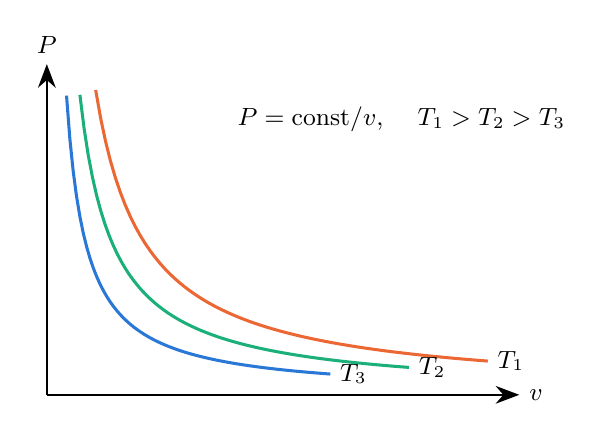
\begin{tikzpicture}
  \draw[axisline] (0,0) -- (6.0,0) node[right, lbl] {$v$};
  \draw[axisline] (0,0) -- (0,4.2) node[above, lbl] {$P$};
  \draw[path2] plot[domain=0.62:5.6, samples=80] (\x, {2.4/\x});
  \draw[path3] plot[domain=0.42:4.6, samples=80] (\x, {1.6/\x});
  \draw[path1] plot[domain=0.25:3.6, samples=80] (\x, {0.95/\x});
  \node[lbl, right] at (5.6,{2.4/5.6}) {$T_1$};
  \node[lbl, right] at (4.6,{1.6/4.6}) {$T_2$};
  \node[lbl, right] at (3.6,{0.95/3.6}) {$T_3$};
  \node[lbl, anchor=west] at (2.3,3.5) {$P = \text{const}/v$, \quad $T_1 > T_2 > T_3$};
\end{tikzpicture}
\end{document}
